\subsection{Refcache: Conflict-free reference counting}

\XXX![AC]{This is verbatim from the (corrected) EuroSys paper.  Update
  to fit.}

Reference counting is critical to many OS functions, and \vm is no
different.  Since two virtual memory regions may share the same physical
pages, such as when forking a process, \vm must have a way
to decide when to free the underlying physical pages.  To do so,
\vm reference counts each physical page, but a simple scheme with a
single counter can result in scalability problems because threads will
contend for the counter.  Likewise, \vm reference counts nodes of its
radix tree to determine when they are empty; a single counter would
cause operations on different parts of the node to contend.

This section introduces \refcache, a novel
reference counting scheme that \vm uses to track and reclaim physical
memory pages and radix tree nodes.
\refcache implements space-efficient, lazy, scalable reference
counting using per-core \emph{reference delta caches}.  \refcache targets
workloads that can tolerate some latency in reclaiming resources and
where increment and decrement operations often occur on the same core
(e.g., the same thread that faulted pages into a mapped memory region
also unmaps that region).  

In contrast with most scalable
reference counting mechanisms (see \S\ref{sec:related}), \refcache
requires space proportional to the sum of the number of reference
counted objects and the number of cores, rather than the product, and
the per-core overhead can be adjusted to trade off space and
scalability by controlling the reference delta cache conflict rate.  This is
important when tracking every physical page in a large multicore
system; at large core counts, typical scalable reference counters
would require more than half of physical memory just to track the
remaining physical memory.  

\refcache batches increment and decrement
operations, reducing cache line movement while offering an adjustable
time bound on when an object will be garbage collected after its
reference count drops to zero.  Objects that are
manipulated from only a single core do not require any per-object cache
line movement and \refcache itself requires only a small constant rate
of cache line movement for global maintenance.

\paragraph{Base \refcache.}
In \refcache, each reference counted object has a global reference
count (much like a regular reference count) and each core also
maintains a local, fixed-size cache of deltas to objects' reference
counts.  Incrementing or decrementing an object's reference count
modifies only the local, cached delta and this delta is periodically
flushed to the object's global reference count.  The true reference
count of an object is thus the sum of its global count and any local
deltas for that object found in the per-core delta caches.  The value of the
true count is generally unknown, but we assume that once it drops to
zero, it will remain zero (in the absence of weak references, which
we discuss later).  \refcache depends on this stability to detect a
zero true count after some delay.

To detect a zero true reference count, \refcache divides time into
periodic \emph{epochs} during which each core flushes all of the
reference count deltas in its cache, applying these updates to the
global reference count of each object.  The last core in an epoch to
finish flushing its cache ends the epoch and all of the cores repeat
this process after some delay (our implementation uses 10ms).  Since
these flushes occur in no particular order and the caches batch
reference count changes, updates to the reference count can be
reordered.  As a result, a zero global reference count does not imply
a zero true reference count.  However, once the true count \emph{is}
zero, there will be no more updates, so if the global reference count
of an object drops to zero and \emph{remains} zero for an entire
epoch, then \refcache can guarantee that the true count is zero
and free the object.  To detect this, the first core that sets an object's
global reference count to zero adds the object to a per-core
\emph{review queue} and reexamines it two epochs later (which
guarantees one complete epoch has elapsed) to decide whether its true
reference count is zero.

\begin{figure*}
  \centering
  \includegraphics[width=\textwidth]{figures/refcache.pdf}
  \caption{\refcache example showing a single object over eight
    epochs.  Plus and minus symbols represent increment and decrement
    operations, dotted lines show when cores flush these to the object's
    global count, and blue circles show when each core flushes its
    local reference cache.  The loops around the global count show
    when the object is in core 0's review queue and
    the red zeroes indicate dirty zeroes.}
  \label{fig:refcache-ex}
\end{figure*}

Figure~\ref{fig:refcache-ex} gives an example of a single object over
the course of eight epochs.  Epoch 1 demonstrates the power of
batching: despite six reference count manipulations spread over three
cores, the object's global reference count is never written to.  The
remaining epochs demonstrate the complications that arise from
batching and the resulting lag between the true reference count and
the global reference count of an object.

Because of the flush order, the two updates in epoch 2 are applied to
the global reference count in the opposite order of how they actually
occurred.  As a result, core 0 observes the global count temporarily
drop to zero when it flushes in epoch 2, even though the true count is
non-zero.  This is remedied as soon as core 1 flushes its increment,
and when core 0 reexamines the object at the beginning of epoch 4,
after all cores have again flushed their delta caches, it can see
that the global count is non-zero; hence, the zero count it observed
was not a true zero and the object should not be freed.

It is not enough for the global reference count to be zero when an
object is reexamined; rather, it must have been zero for the entire
epoch.  For example, core 0 will observe a zero global reference count
at the end of epoch 4, and again when it reexamines the object in
epoch 6.  However, the true count is not zero, and the global
reference count was temporarily non-zero during the epoch.  We call
this a \emph{dirty} zero and in this situation \refcache will
queue the object to be examined again two epochs later, in epoch 8.

\paragraph{Weak references.}
As described, \refcache is well suited to reference counts that track
the true number of references to an object, since there is no danger
of the count going back up once the object becomes unreachable.
However, operating systems often need untracked references to objects;
for example, OS caches track objects that may be deleted at any time,
and may even need to bring an object's reference count back up from
zero.  \vm's radix tree has similar requirements.  To support such
uses, we extend \refcache with \emph{weak references}, which provide a
\code{tryget} operation that will either increment the object's
reference count (even if it has reached zero) and return the object,
or will indicate that the object has already been deleted.

A weak reference is simply a pointer marked with a ``dying'' bit,
along with a back-reference from the referenced object.  When an
object's global reference count initially reaches zero, \refcache sets
the weak reference's dying bit.  After this, \code{tryget} can
``revive'' the object by atomically clearing the dying bit and
fetching the pointer value, and then incrementing the object's
reference count as usual.  When \refcache decides to free an object,
it first atomically clears both the dying bit and the pointer in the
weak reference.  If this succeeds, it can safely delete the object.
If this fails, it reexamines the object again two epochs later.  In a
race between \code{tryget} and deletion, which operation succeeds is determined
by which clears the dying bit first.

\paragraph{Algorithm.}
The pseudocode for \refcache is given in
Figure~\ref{fig:refcache-code}.  Each core maintains a hash table
storing its reference delta cache and the review queue that tracks
objects whose global reference counts reached zero.  A core reviews an
object after two epoch boundaries have passed so it can guarantee
that all cores have flushed their
reference caches at least once.

\XXX![AC]{Make pseudo-code formatting consistent with rule chapter.}

\begin{figure}
  \begin{tabbing}
    \quad\=\quad\=\quad\=\quad\=\quad\=\quad\=\kill
    inc(obj): \+\\
      if local cache[hash(obj)].obj $\ne$ obj: \+\\
        evict(local cache[hash(obj)]) \\
        local cache[hash(obj)] $\gets$ $\langle$obj, 0$\rangle$ \-\\
      local cache[hash(obj)].delta += 1 \\
    \-\\
    tryget(weakref): \+\\
      do: \+\\
        $\langle$obj, dying$\rangle$ $\gets$ weakref \-\\
      while weakref.cmpxchng($\langle$obj, dying$\rangle$,
        $\langle$obj, false$\rangle$) fails \\
      if obj is not null: \+\\
        inc(obj) \-\\
      return obj \\
    \-\\
    flush(): \+\\
      evict all local cache entries and clear cache \\
      update the current epoch \\
    \-\\
    evict(obj, delta): \+\\
      % If this condition is true, then the locked region would be a
      % no-op, but why is it safe to do it without the lock?  The
      % danger is that the read of refcnt will slip in the middle of
      % another region that modified refcnt with obj locked.  evict
      % is the only place this happens and it does only a single write
      % to refcnt.  Assuming both this read and that write are
      % atomic, then we can consider this check atomic with the entire
      % locked region in the competing evict.
      if delta = 0 and obj.refcnt $\ne$ 0: return \\
      with obj locked: \+\\
        obj.refcnt $\gets$ obj.refcnt + delta \\
        if obj.refcnt = 0: \+\\
          if obj is not on any review queue: \+\\
            obj.dirty $\gets$ false \\
            obj.weakref.dying $\gets$ true \\
            add $\langle$obj, epoch$\rangle$ to the local review
            queue \-\\
          else: \+\\
            obj.dirty $\gets$ true \\
    \-\-\-\-\\
    review(): \+\\
      for each $\langle$obj, objepoch$\rangle$ in local review queue: \+\\
        if epoch $<$ objepoch + 2: continue \\
        with obj locked: \+\\
          remove obj from the review queue \\
          if obj.refcnt $\ne$ 0: \+\\
            obj.weakref.dying $\gets$ false \-\\
          else if obj.dirty or obj.weakref.cmpxchng(%
                $\langle$obj, true$\rangle$, \+\+\\
                $\langle$null, false$\rangle$) fails: \-\\
            obj.dirty $\gets$ false \\
            obj.weakref.dying $\gets$ true \\
            add $\langle$obj, epoch$\rangle$ to the local review queue \-\\
          else: \+\\
            free obj
  \end{tabbing}
  \vspace{-1em}                 % No idea where this space comes from
  \caption[\refcache algorithm.]
  {\refcache algorithm.  Each core calls \code{flush} and \code{review}
    periodically.  \code{evict} may be called by \code{flush} or because of a
    collision in the reference cache.  \code{dec} is identical to \code{inc} except
    that it decrements the locally cached delta.}
  \label{fig:refcache-code}
\end{figure}

All of the functions in Figure~\ref{fig:refcache-code} execute with
preemption disabled, meaning they are atomic with respect to each
other on a given core, which protects the consistency of per-core data
structures.  Individual objects are protected by fine-grained locks
that protect the consistency of the object's fields.

For epoch management, our current implementation uses a barrier scheme
that tracks a global epoch counter, per-core epochs, and a count of
how many per-core epochs have reached the current global epoch.  This
scheme suffices for our benchmarks, but more scalable schemes are
possible, such as the tree-based quiescent state detection used
by Linux's hierarchical RCU implementation~\cite{lwn:treercu}.

\paragraph{Discussion.}
\refcache trades latency for scalability by batching increment and
decrement operations in per-core caches.  As a result, except when
there are conflicts in the reference delta cache, increment and
decrement operations do not share cache lines with other cores and
communication is necessary only when these caches are periodically
reconciled.  Furthermore, because \refcache uses per-core caches
rather than per-core counts, it is more space-efficient than other
scalable reference counting techniques.  While not all uses of
reference counting can tolerate \refcache's latency, its scalability
and space-efficiency are well suited to the requirements of \vm.

\XXX[Austin]{Design alternatives: token-passing or broadcast IPI for
epoch detection; lock-free versus fine-grained locking?}
